% Made with matchcha.io---strong recommendation from me! :)

\tikzset{every picture/.style={line width=0.75pt}} %set default line width to 0.75pt        

\makebox[\textwidth][c]{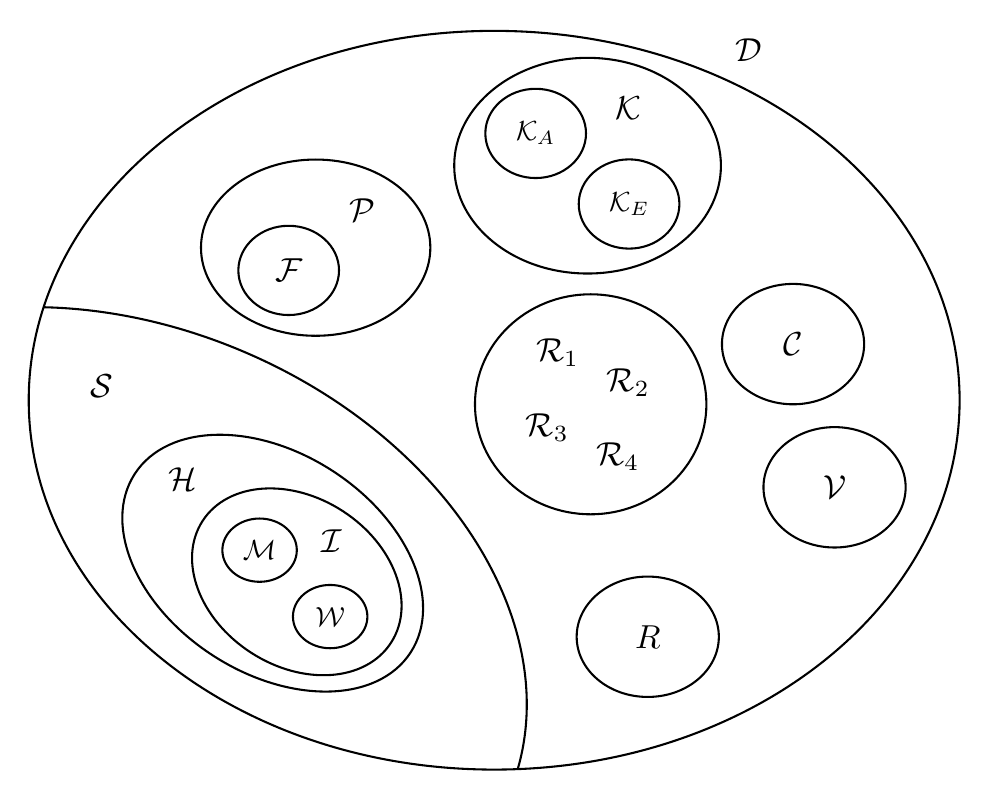
\begin{tikzpicture}[x=0.75pt,y=0.75pt,yscale=-1,xscale=1,scale=1,every node/.style={scale=1}]
%uncomment if require: \path (0,721.921875); %set diagram left start at 0, and has height of 721.921875

%Shape: Ellipse [id:dp9100065238827619] 
\draw   (98,300.96) .. controls (98,202.68) and (198.4,123) .. (322.25,123) .. controls (446.1,123) and (546.5,202.68) .. (546.5,300.96) .. controls (546.5,399.25) and (446.1,478.92) .. (322.25,478.92) .. controls (198.4,478.92) and (98,399.25) .. (98,300.96) -- cycle ;
%Shape: Ellipse [id:dp10388374342633644] 
\draw   (181,227.46) .. controls (181,204.01) and (205.74,185) .. (236.25,185) .. controls (266.76,185) and (291.5,204.01) .. (291.5,227.46) .. controls (291.5,250.91) and (266.76,269.92) .. (236.25,269.92) .. controls (205.74,269.92) and (181,250.91) .. (181,227.46) -- cycle ;
%Shape: Ellipse [id:dp27736097111625835] 
\draw   (199,238.42) .. controls (199,226.55) and (209.86,216.92) .. (223.25,216.92) .. controls (236.64,216.92) and (247.5,226.55) .. (247.5,238.42) .. controls (247.5,250.3) and (236.64,259.92) .. (223.25,259.92) .. controls (209.86,259.92) and (199,250.3) .. (199,238.42) -- cycle ;
%Shape: Ellipse [id:dp7888799168086817] 
\draw   (303,187.96) .. controls (303,159.26) and (331.77,136) .. (367.25,136) .. controls (402.73,136) and (431.5,159.26) .. (431.5,187.96) .. controls (431.5,216.66) and (402.73,239.92) .. (367.25,239.92) .. controls (331.77,239.92) and (303,216.66) .. (303,187.96) -- cycle ;
%Shape: Ellipse [id:dp4804121479534271] 
\draw   (363,206.42) .. controls (363,194.55) and (373.86,184.92) .. (387.25,184.92) .. controls (400.64,184.92) and (411.5,194.55) .. (411.5,206.42) .. controls (411.5,218.3) and (400.64,227.92) .. (387.25,227.92) .. controls (373.86,227.92) and (363,218.3) .. (363,206.42) -- cycle ;
%Shape: Ellipse [id:dp0795716353230258] 
\draw   (318,172.42) .. controls (318,160.55) and (328.86,150.92) .. (342.25,150.92) .. controls (355.64,150.92) and (366.5,160.55) .. (366.5,172.42) .. controls (366.5,184.3) and (355.64,193.92) .. (342.25,193.92) .. controls (328.86,193.92) and (318,184.3) .. (318,172.42) -- cycle ;
%Shape: Ellipse [id:dp12618348576003102] 
\draw   (432,273.92) .. controls (432,257.91) and (447.33,244.92) .. (466.25,244.92) .. controls (485.17,244.92) and (500.5,257.91) .. (500.5,273.92) .. controls (500.5,289.94) and (485.17,302.92) .. (466.25,302.92) .. controls (447.33,302.92) and (432,289.94) .. (432,273.92) -- cycle ;
%Shape: Ellipse [id:dp8799691211755756] 
\draw   (452,342.92) .. controls (452,326.91) and (467.33,313.92) .. (486.25,313.92) .. controls (505.17,313.92) and (520.5,326.91) .. (520.5,342.92) .. controls (520.5,358.94) and (505.17,371.92) .. (486.25,371.92) .. controls (467.33,371.92) and (452,358.94) .. (452,342.92) -- cycle ;
%Shape: Ellipse [id:dp824996442524188] 
\draw   (362,414.92) .. controls (362,398.91) and (377.33,385.92) .. (396.25,385.92) .. controls (415.17,385.92) and (430.5,398.91) .. (430.5,414.92) .. controls (430.5,430.94) and (415.17,443.92) .. (396.25,443.92) .. controls (377.33,443.92) and (362,430.94) .. (362,414.92) -- cycle ;
%Shape: Ellipse [id:dp8272383634329143] 
\draw   (313,302.92) .. controls (313,273.65) and (337.96,249.92) .. (368.75,249.92) .. controls (399.54,249.92) and (424.5,273.65) .. (424.5,302.92) .. controls (424.5,332.19) and (399.54,355.92) .. (368.75,355.92) .. controls (337.96,355.92) and (313,332.19) .. (313,302.92) -- cycle ;
%Shape: Arc [id:dp39537977602891705] 
\draw  [draw opacity=0] (105.32,256.16) .. controls (135.93,256.87) and (168.45,263.64) .. (200.4,277.07) .. controls (297.72,317.98) and (354.69,406) .. (333.59,478.73) -- (143.5,412.42) -- cycle ; \draw   (105.32,256.16) .. controls (135.93,256.87) and (168.45,263.64) .. (200.4,277.07) .. controls (297.72,317.98) and (354.69,406) .. (333.59,478.73) ;
%Shape: Ellipse [id:dp5287011551360823] 
\draw   (149.07,336.49) .. controls (164.96,311.91) and (207.6,311.22) .. (244.32,334.95) .. controls (281.04,358.69) and (297.92,397.86) .. (282.03,422.44) .. controls (266.14,447.02) and (223.49,447.71) .. (186.77,423.97) .. controls (150.06,400.24) and (133.18,361.07) .. (149.07,336.49) -- cycle ;
%Shape: Ellipse [id:dp015166695228427951] 
\draw   (181.78,359.11) .. controls (193.96,340.26) and (224.16,338.12) .. (249.23,354.32) .. controls (274.3,370.53) and (284.75,398.94) .. (272.56,417.79) .. controls (260.38,436.64) and (230.18,438.78) .. (205.11,422.58) .. controls (180.04,406.37) and (169.59,377.96) .. (181.78,359.11) -- cycle ;
%Shape: Ellipse [id:dp4822793325306267] 
\draw   (191.3,373.21) .. controls (191.3,364.79) and (199.33,357.96) .. (209.23,357.96) .. controls (219.14,357.96) and (227.17,364.79) .. (227.17,373.21) .. controls (227.17,381.63) and (219.14,388.45) .. (209.23,388.45) .. controls (199.33,388.45) and (191.3,381.63) .. (191.3,373.21) -- cycle ;
%Shape: Ellipse [id:dp37988107849014874] 
\draw   (225.3,405.21) .. controls (225.3,396.79) and (233.33,389.96) .. (243.23,389.96) .. controls (253.14,389.96) and (261.17,396.79) .. (261.17,405.21) .. controls (261.17,413.63) and (253.14,420.45) .. (243.23,420.45) .. controls (233.33,420.45) and (225.3,413.63) .. (225.3,405.21) -- cycle ;

% Text Node
\draw (133,294) node [scale=1.2]  {$\mathcal{S}$};
% Text Node
\draw (244,369) node [scale=1.2]  {$\mathcal{I}$};
% Text Node
\draw (209.23,373.21) node [scale=1]  {$\mathcal{M}$};
% Text Node
\draw (243.23,405.21) node [scale=1]  {$\mathcal{W}$};
% Text Node
\draw (172.23,339.21) node [scale=1.2]  {$\mathcal{H}$};
% Text Node
\draw (396.25,414.92) node [scale=1.2]  {$\mathbb{R}$};
% Text Node
\draw (352.8,278.27) node [scale=1.2]  {$\mathcal{R}_{1}$};
% Text Node
\draw (386.8,292.27) node [scale=1.2]  {$\mathcal{R}_{2}$};
% Text Node
\draw (347.8,314.27) node [scale=1.2]  {$\mathcal{R}_{3}$};
% Text Node
\draw (381.8,328.27) node [scale=1.2]  {$\mathcal{R}_{4}$};
% Text Node
\draw (386.8,160.27) node [scale=1.2]  {$\mathcal{K}$};
% Text Node
\draw (342.25,172.42) node [scale=1]  {$\mathcal{K}_{A}$};
% Text Node
\draw (387.25,206.42) node [scale=1]  {$\mathcal{K}_{E}$};
% Text Node
\draw (466.25,273.92) node [scale=1.2]  {$\mathcal{C}$};
% Text Node
\draw (486.25,342.92) node [scale=1.2]  {$\mathcal{V}$};
% Text Node
\draw (258.8,209.27) node [scale=1.2]  {$\mathcal{P}$};
% Text Node
\draw (223.25,238.42) node [scale=1.2]  {$\mathcal{F}$};
% Text Node
\draw (444.8,132.27) node [scale=1.2]  {$\mathcal{D}$};


\end{tikzpicture}}

\makebox[\textwidth][c]{\begin{tabular}{c c l}
   & & \\
   $\mathcal{D}$  & & The full \textit{domain} of EL individuals; the union of all following sets \\
   $\mathcal{S}$  & & Possible situations, a.k.a. \textit{episodes} \\
   %$\mathcal{H}$  & & Informationally-maximal episodes, a.k.a. \textit{exhaustive situations} \\
   %$\mathcal{I}$  & & Spatially-maximal exhaustive situations, a.k.a. \textit{possible times}, a.k.a intervals \\
   %$\mathcal{W}$  & & Spatiotemporally-maximal intervals, a.k.a. \textit{possible worlds} \\
   %$\mathcal{M}$  & & Spatially-maximal, temporally-minimal intervals, a.k.a. \textit{moments of time} \\
   $\mathcal{P}$  & & \textit{Propositions} \\
   $\mathcal{F}$  & & Consistent propositions, a.k.a. \textit{facts} \\
   $\mathcal{K}$  & & \textit{Kinds of individuals} \\
   $\mathcal{K}_{A}$  & & \textit{Kinds of actions} \\
   $\mathcal{K}_{E}$  & & \textit{Kinds of episodes} \\
   $\mathcal{C}$  & & \textit{Collections} \\
   $\mathcal{V}$  & & \textit{$n$-tuples, $n \geq 2$} \\
   $\mathbb{R}$  & & \textit{The real numbers} \\
   $\mathcal{R}_{1 \leq n \leq 4}$  & & \textit{$n$-dimensional regions}, containing subsets of $\mathbb{R}_{n}$
   %& & Note that $\mathcal{R}_{4}$, which represents space-time regions, contains some unconnected \\
   %& & space-time trajectories; these trajectories describe the time and place of episodes.
\end{tabular}}